\section{Reducción de dimensiones}\label{sec:dimensionalityReduction}

\begin{frame}
    \frametitle{Análisis de Componentes Principales}

    \begin{figure}[!h]
        \centering
        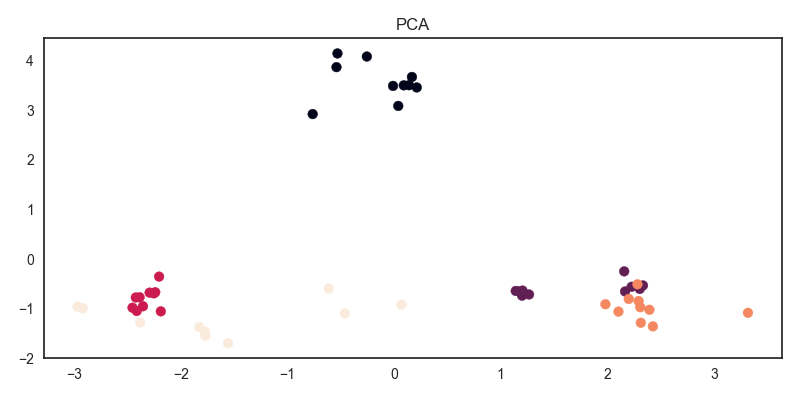
\includegraphics[width=\textwidth]{pca.png}
    \end{figure}

    {\footnotesize
    Resultado de aplicar PCA para reducir a dos las dimensiones de los MFCC de un conjunto de sonidos de cinco especies animales.
    }
\end{frame}

\begin{frame}
    \frametitle{Manifold Learning}

    \begin{columns}
        \column{0.5\textwidth}

        \begin{itemize}
            \item<2-> \textbf{Multi-dimensional Scaling (MDS)}
            \begin{equation*}
                \sum_{i=1}^{N}\sum_{j=i+1}^{N}{d_{ij} - \hat{d}_{ij}}
            \end{equation*}
            \item<3-> \textbf{Isomap} \\
            MDS sobre la \textit{distancia geodésica}
            \item<4-> \textbf{Locally Linear Embedding (LLE)}
        \end{itemize}

        \column{0.5\textwidth}

        \begin{figure}[!h]
            \centering
            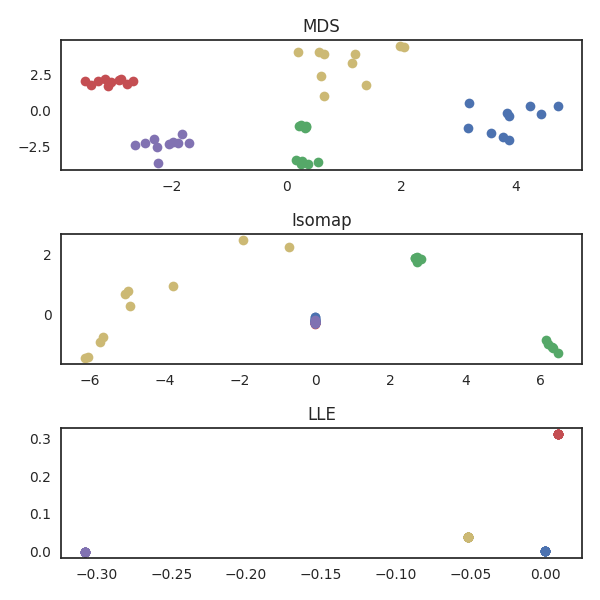
\includegraphics[width=\textwidth]{manifold-learning-vertical.png}
        \end{figure}

    \end{columns}
\end{frame}